\documentclass[a4paper]{scrartcl}

\usepackage{float}
\usepackage{tikz}
\usetikzlibrary{arrows,automata}
\usepackage{pgf}
\usepackage[utf8]{inputenc} % this is needed for umlauts
\usepackage[ngerman]{babel} % this is needed for umlauts
\usepackage[T1]{fontenc}    % this is needed for correct output of umlauts in pd
\usepackage{amssymb}
\usepackage{amsmath}
\usepackage{mathrsfs}
\usepackage{dsfont}
\usepackage{graphicx}
\usepackage{fancyhdr}
\usepackage{lastpage}
\usepackage{imakeidx}
\setlength{\parskip}{\medskipamount}
\setlength{\parindent}{0pt}
\usepackage{enumitem}
\usepackage{hyperref}

%%%%%%%%%%%%%%%%%%%%%%%%
% Kopf- und Fusszeilen %
%%%%%%%%%%%%%%%%%%%%%%%%
\pagestyle{fancy}
\lhead{
        Maximilian Roth
}
\chead{Logik-Tutorat Lösungen Blatt 3\\}
\rhead{
        \today{} \\
        Seite \thepage{} von \pageref{LastPage}\\
        
}
\lfoot{}
\cfoot{}
\rfoot{} 

%%%%%%%%%%%%%%%%%%%%%%%%
% Anfang des Dokuments %
%%%%%%%%%%%%%%%%%%%%%%%%

\begin{document}
\section*{Disclaimer}%
\label{sec:disclaimer}
Auch in diesem Dokument können sich Fehler befinden!\\
Sie sind nicht die Musterlösung der Aufgaben, sondern selbst erstellte Lösungen.\\

Als generelle Lektüre kann ich nur das Skript von Markus Junker aus dem WS 17/18 empfehlen:\\
\url{http://home.mathematik.uni-freiburg.de/junker/skripte/InfoLogik.pdf}\\
Hier ist vieles sehr genau und verständlich erklärt.

\section*{}%
\label{sec:aufgabe_1}

    \begin{figure}[H]
        \centering
        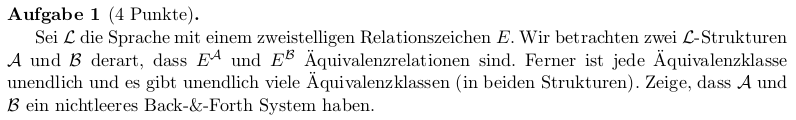
\includegraphics[scale=0.6]{./A-1.png}
        \label{fig:}
    \end{figure} 

    Siehe auch Aufbau Back \& Forth am Ende des Dokuments.~\ref{sec:aufbau_back_forth}

    \underline{Beweis:}\\
    Wir sollen zeigen, dass es ein nicht leeres Back and Forth System gibt, also müssen wir uns zuerst eines aussuchen.\\
    \\Hierfür empfiehlt es sich zuerst mit folgendem S anzufangen:\\
    $S = \{F: \mathfrak{C} \rightarrow \mathfrak{D} \mathscr{L}-Isomorphismus| \mathfrak{C} \subset \mathfrak{A}, \mathfrak{D} \subset \mathfrak{B},
    \text{ wobei  }\mathfrak{C}, \mathfrak{D} \text{ endlich erzeugt}\}$ ist.\\
    Mit $\mathfrak{C} \subset \mathfrak{A}$ ist gemeint, dass $\mathfrak{C}$ Unterstruktur von $\mathfrak{A}$ ist.\\

    \\Zeigen wir also nun, dass S ein nichtleeres Back and Forth System ist. 

    \begin{itemize}
        \item S ist nichtleer\\
            Sei gegeben: $\mathfrak{C} = (\{c\}, \{E^\mathfrak{C}\}), \mathfrak{D} = (\{d\}, \{E^\mathfrak{D}\})$\\
            \\Dann gilt, dass $F: \{c\} \rightarrow \{d\}, c \mapsto d$ Isomorphismus ist
            \\(Die von \{c\} und \{d\} erzeugten Mengen sind wieder \{c\} bzw. \{d\} und offensichtlich endlich erzeugt),\\
            da F klar bijektiv und E in beiden Strukturen Äquivalenzerelartion ist, womit F auch starker $\mathscr{L}$-Hom. ist.\\
            $\Rightarrow$ S ist nicht leer.\\

        \item S ist Back & Forth System\\
            \begin{itemize}
                \item \framebox{Back:}\\
                    Sei $F \in S$ und $b \in B\backslash Im(F)$\\                  
                    \\1. Falls dieses b in Äquivalenzerelation mit einem b' aus dem Bild Im(F) steht.\\
                    Suchen wir ein $a \in A$ für das gilt $(a, F^{-1}(b')) \in E^{\mathfrak{A}}$ und setzen F'(a) = b.\\
                    \\2. Falls dieses b in keiner Äquivalenzerelation steht darf das dazugehörige a dies auch nicht tun.\\
                    Also suchen wir ein a für das gilt: $(a, a') \notin E^{\mathfrak{A}}, \forall a' \in Dom(F)$ und setzen F'(a) = b.\\

                \item \framebox{Forth:}\\
                    Sei $F \in S$ und $a \in A\backslash Dom(F)$\\
                    \\1. Falls a in einer Äquivalenzerelation mit einem a' steht.\\
                    Dann suchen wir ein b, sodass gilt $(b, F(a')) \in E^{\mathfrak{B}}$ und setzen F'(a) = b.\\
                    \\2. Falls a in keiner Äquivalenzerelation steht.\\
                    Dann suchen wir ein b, sodass $(b, b') \notin E^{\mathfrak{B}}, \forall b' \in Im(F)$ und setzen F(a) = b.\\
            \end{itemize}

            $\Rightarrow$ S ist Back \& Forth System.\\
    \end{itemize}
    $\Rightarrow$ S ist nichtleeres Back \& Forth System.
    



\section*{}%
\label{sec:aufgabe_2}

    \begin{figure}[H]
        \centering
        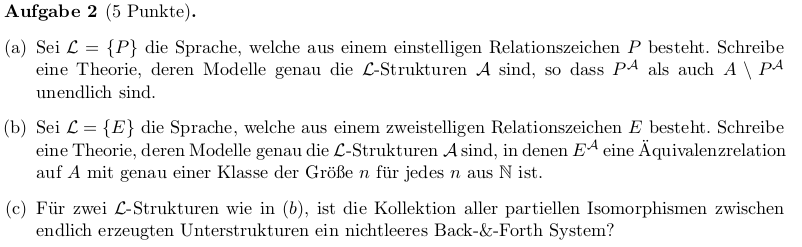
\includegraphics[scale=0.6]{./A-2.png}
        \label{fig:}
    \end{figure}

    Eine Theorie ist eine Menge T von $\mathscr{L}$-Aussagen.\\
    Eine $\mathscr{L}$-Aussage wiederum ist eine Formel ohne freie Variablen,\\
    das heißt entweder gibt es keine Individuenvariablen oder sie sind im Wirkungsbereich
    eines Quantors.\\

    \begin{itemize}
        \item a)\\
            $T = A_1 \cup A_2$\\
            $A_1 = \{\exists x_1 \dots \exists x_n (\bigwedge_{i \neq j}(\neg x_i \doteq x_j \land P(x_i,x_j))) | n \in \mathds{N}\}$\\
            Also keine zwei Variablen sind gleich und alle n sind in Relation\\
            $\Rightarrow$ Es gibt min n Elemente in P $\forall n \in \mathds{N}$\\
            $\Rightarrow$ Es gibt unendlich viele Elemente in P\\
            \\$A_2 = \{\exists x_1 \dots \exists x_n (\bigwedge_{i \neq j}(\neg x_i \doteq x_j \land \neg P(x_i,x_j))) | n \in \mathds{N}\}$\\
            Es sind also mindestens n Elemente nicht in P $\forall n \in \mathds{N}$\\
            $\Rightarrow$ Es gibt unendlich viele Elemente, die nicht in P liegen.\\
            \\Aus $T = A_1 \cup A_2$ folgt, dass unendlich viele Elemente in P sind und unendlich viele es nicht sind.\\

        \item b)\\
            Zunächst die Aussagen für eine Äquivalenzerelation:\\
            $A_{reflexif} = \{\forall x (E(x,x))\}$\\
            $A_{symmetrisch} = \{\forall x \forall y (E(x,y) \rightarrow E(y,x))\}$\\
            $A_{transitiv} = \{\forall x \forall y \forall z ((E(x,y) \land E(y,z)) \rightarrow E(x,z))\}$\\
            \\Und nun die für die n-elementigen Äquivalenzklassen $\forall n \in \mathds{N}$:\\
            $A_n = \{\forall x_1,...,\forall x_n,\forall a (\bigwedge_{i \neq j} (\neg x_1 \doteq x_j)  \land E(x_i,x_j) \land (\neg a \doteq x_i) \land \neg E(a, x_i))\}$\\
            \\Auf deutsch:\\
            Es gibt n verschiedene Elemente der Form $x_i$.\\
            Alle $x_i$ sind in einer Relation miteinander.\\
            Es gibt ein a, dass von allen $x_i$ verschieden ist.\\
            a steht mit keinem $x_i$ in Relation.\\
            \\Daraus folt in $A_i$ gibt es \underline{genau} i verschiedene Elemente,
            \\die in Relation zu einander stehen keines mehr keines weniger.\\

            \\Mit $T = A_{reflexif} \cup A_{symmetrisch} \cup A_{transitiv} \cup A_i, \forall i \in \mathds{N}$ besitzt T genau die nötigen Eigenschaften.\\

        \item c)\\
            Bei diesem Back \& Forth System haben wir ein S gegeben:\\
            S = \{partieller Iso. mit endl. erz. Unterstrukturen wie in b)\} und sollen zeigen,\\
            dass es kein nichtleeres B \& F System gibt.\\

           \\\underline{Beweis:}\\
            Angenommen $\mathfrak{A}, \mathfrak{B}$ sind Strukturen wie in b) beschrieben, also $\mathfrak{A}, \mathfrak{B} \models T_{b)}$\\
            Und sei F bereits folgendermaßen: F(a) = b, wobei die Äquivalenzklasse von a \{a,a'\} und die von b \{b\} ist.\\

            \\Forth würde nun versuchen ein passendes $b' \in B$ für a' zu finden, sodass die Isomorphie erhalten bleibt, also (u.a.) gilt:\\
            $(a, a') \in E^{\mathfrak{A}} \Leftrightarrow (F(a),F(a')) = (b, b') \in E^{\mathfrak{B}}$.\\
            Es gibt aber nur dieses eine b in der Äquivalenzklasse und für eine Isomorphie muss Injektivität gelten.\\
            \\$\Rightarrow$ Es gibt also kein F', dass auch a' entsprechend abbildet und in S liegt.\\
            $\Rightarrow$ S ist nicht Back \& Forth System (S ist trotzdem nichtleer).



    \end{itemize}


\section*{}%
\label{sec:aufgabe_3}

    \begin{figure}[H]
        \centering
        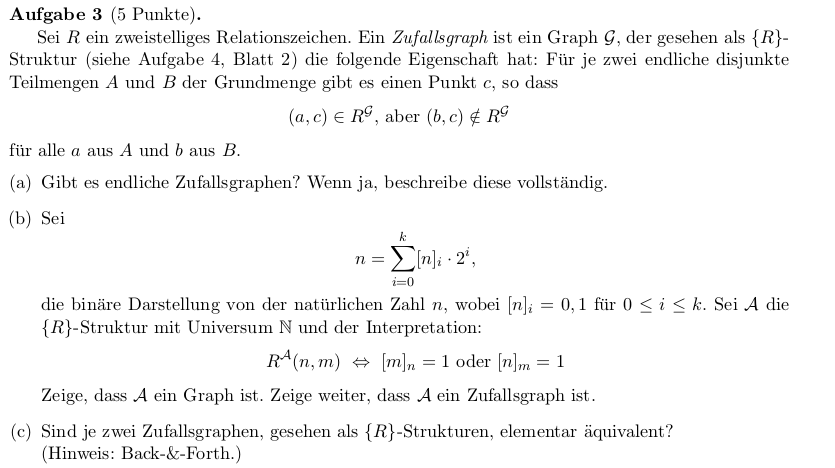
\includegraphics[scale=0.6]{./A-3.png}
        \label{fig:}
    \end{figure}

\section*{}%
\label{sec:aufgabe_4}

    \begin{figure}[H]
        \centering
        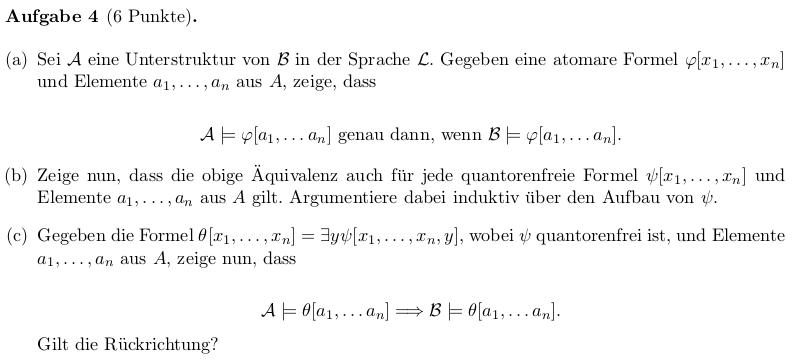
\includegraphics[scale=0.6]{./A-4.png}
        \label{fig:}
    \end{figure}


\section*{Aufbau Back \& Forth}%
\label{sec:aufbau_back_forth}
    Das finden eines nichtleeren Back \& Forth Systems S wird dazu genutzt, um zu zeigen, dass zwei Strukturen elementar äquivalent sind.
    \begin{figure}[H]
        \centering
        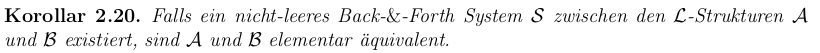
\includegraphics[scale=0.6]{./B&F-EA.png}
        \label{fig:}
    \end{figure}

    Das heißt, wenn eine eine partielle elementare Abbildung von der einen in die andere Struktur existiert:
    
    \begin{figure}[H]
        \centering
        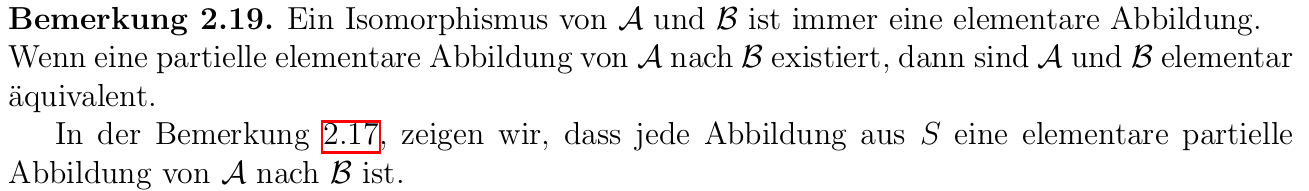
\includegraphics[scale=0.3]{./B&F-PEA.png}
        \label{fig:}
    \end{figure}

    Was wiederum der fall ist, wenn folgendes gilt:

    \begin{figure}[H]
        \centering
        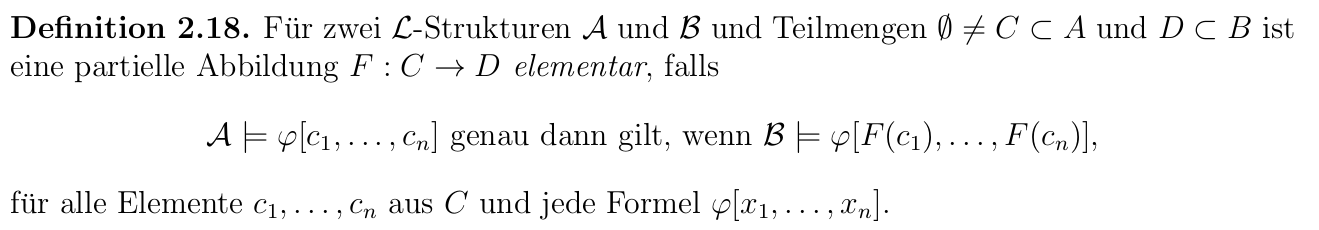
\includegraphics[scale=0.3]{./B&F-E.png}
        \label{fig:}
    \end{figure}

    Also suchen wir stets (falls nicht gegeben) eine Kollektion S mit den Eigenschaften:\\

    $S = \{F: \mathfrak{C} \rightarrow \mathfrak{D} \mathscr{L}-Isomorphismus| \mathfrak{C} \subset \mathfrak{A}, \mathfrak{D} \subset \mathfrak{B},
    \text{ wobei  }\mathfrak{C}, \mathfrak{D} \text{ endlich erzeugt}\}$ ist.\\
    Mit $\mathfrak{C} \subset \mathfrak{A}$ ist gemeint, dass $\mathfrak{C}$ Unterstruktur von $\mathfrak{A}$ ist.\\

    Falls dieses S kein nichtleeres Back \& Forth System ist, können wir ein weiter eingeschränktes S suchen.\\
    Hier hängt die Einschränkung vom konkreten Fall ab, schaut einfach, wo das Problem für euer erstes S lag.\\
    Es kann natürlich aus sein, dass keins existiert, wenn dies der Fall ist seht ihr das aber in der Regel schnell.\\

    Habt ihr ein S, dann zeigt die nötigen Eigenschaften:\\
    \begin{itemize}
        \item S ist nichtleer\\
        \item S ist Back \& Forth System\\
            \begin{itemize}
                \item \framebox{Back:}\\
                    Sei $F \in S$, also F bildet von C nach D isomorph ab und gelte $b \in B\backslash Im(F)$.\\
                    Dann muss für dieses beliebige b gelten, dass ein $a \in A\backslash Dom(F)$ und damit ein F'$ existiert mit:\\
                    \\$F': A\cup \{a\} \rightarrow B \cup \{b\} $,\\
                    \\also ein F'(a) = b, welches nur für a anders abbildet und die Isomorphie-\\Eigenschaften erhält.\\
                    Wenn b also mit x in einer Relation war,\\
                    so muss dies auch für a und $F'^{-1}(x)$ der Fall sein usw.\\
                    \\Wenn wir zeigen können, dass wir immer ein solches a finden ist Back fertig, falls nicht stimmt S nicht.\\
                
                \item \framebox{Forth:}\\
                    Ziemlich gleich zu Back\\
                    \\$F \in S$ und $a \in A\backslash Dom(F)$ beliebig\\
                    Falls wir ein $b \in B\backslash Im(F)$ finden, für das wir F'(a) = b setzen können\\
                    (wieder ist F' nur bei a zu F unterschiedlich) und dass die Isomorphie behält sind wir mit Forth fertig.\\

            \end{itemize}

    \end{itemize}

    Haben wir beides erfolgreich gezeigt gibt es ein nichtleeres Back \& Forth System und die Strukturen sind elementar äquivalent.\\


\end{document}

